\documentclass[border=3pt]{standalone}
\usepackage{tikz}
\usetikzlibrary{arrows.meta,calc,positioning}
\tikzset{pin/.style={-{Stealth[length=5pt]}},
  blk/.style={draw, thick, minimum height=14mm, align=center, font=\sffamily\small}}
\begin{document}
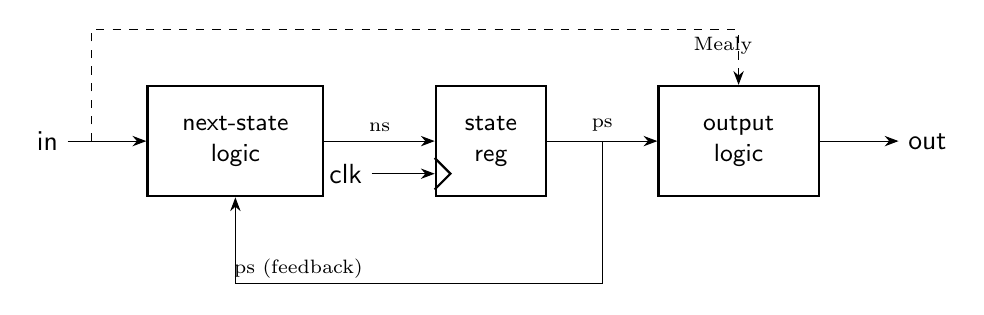
\begin{tikzpicture}[font=\sffamily, node distance=14mm]
  \node[blk, text width=20mm] (ns) {next-state\\logic};
  \node[blk, right=of ns, minimum width=14mm] (reg) {state\\reg};
  \node[blk, right=of reg, text width=18mm] (out) {output\\logic};
  % clock triangle on state reg
  \draw[thick] ($(reg.south west)+(0,1mm)$) -- ++(2mm,2mm) -- ++(-2mm,2mm);
  % main path
  \draw[pin] ($(ns.west)+(-10mm,0)$) node[left]{in} -- (ns.west);
  \draw[pin] (ns.east) -- node[above,font=\scriptsize]{ns} (reg.west);
  \draw[pin] (reg.east) -- node[above,font=\scriptsize]{ps} (out.west);
  \draw[pin] (out.east) -- ++(10mm,0) node[right]{out};
  % feedback ps -> ns
  \coordinate (fb) at ($(reg.east)!0.5!(out.west)$);
  \draw (fb) |- ($(ns.south)+(0,-11mm)$);
  \draw[pin] ($(ns.south)+(0,-11mm)$) -- (ns.south);
  \node[font=\scriptsize] at ($(ns.south)+(8mm,-9mm)$){ps (feedback)};
  % clk
  \draw[pin] ($(reg.south west)+(-8mm,3mm)$) node[left]{clk} -- ($(reg.south west)+(0,3mm)$);
  % Mealy dashed path: in -> output logic (over the top)
  \coordinate (tap) at ($(ns.west)+(-7mm,0)$);
  \draw[pin, dashed] (tap) |- ($(out.north)+(0,7mm)$) -- (out.north);
  \node[font=\scriptsize] at ($(out.north)+(-2mm,5mm)$){Mealy};
\end{tikzpicture}
\end{document}
